\usepackage{amsmath}
\usepackage{amsfonts}
\usepackage{graphicx}
%\usepackage[square,numbers]{natbib}
%\bibliographystyle{abbrvnat}
%\usepackage{amsmath,amssymb,amsfonts,mathtools,amsthm,amsopn}
\usepackage{mathrsfs}
\usepackage{algorithmic}
\usepackage{graphicx}
\usepackage{textcomp}
\usepackage{comment}
\usepackage{wrapfig}
%\usepackage[usenames,dvipsnames,svgnames,table,xcdraw]{xcolor}
%\newcommand{\overbar}[1]{\mkern 1.5mu\overline{\mkern-1.5mu#1\mkern-1.5mu}\mkern 1.5mu}
%\def\BibTeX{{\rm B\kern-.05em{\sc i\kern-.025em b}\kern-.08em
%	T\kern-.1667em\lower.7ex\hbox{E}\kern-.125emX}}
\usepackage{tikz}
%\usepackage{pgfplots}

\usepackage[calc]{adjustbox}
\usepackage{wrapfig}
\usepackage{multicol}\setlength{\multicolsep}{3pt plus 2pt minus 1pt}
%\usepackage[shrink = 15, stretch = 10]{microtype}

\usepackage{csvsimple}
\definecolor{darkgray}{rgb}{0.3, 0.3, 0.3}
\definecolor{darkgreen}{rgb}{0.0, 0.7, 0.3}
\definecolor{darkblue}{rgb}{0.0, 0.3, 0.8}
\definecolor{darkred}{rgb}{0.7, 0.1, 0.1}
\definecolor{darkpurple}{rgb}{0.4, 0.0, 0.6}
\definecolor{darkgold}{rgb}{0.8, 0.6, 0}

%\newcolumntype{P}[1]{>{\centering\arraybackslash}p{#1}}
%\newlength{\strutheight}
%\settoheight{\strutheight}{\strut}
% \setlength{\parskip}{\baselineskip}
%\pagestyle{empty}
%\raggedbottom
%\usepackage{needspace}
%\usepackage{enumitem}

%%% Caligraphic fonts packages
\usepackage[scr=boondox]{mathalfa}

\usepackage{alltt}

\newcommand{\gcu}[1]{\textcolor[rgb]{1.00,0.00,0.00}{#1}} %update
\newcommand{\gcn}[1]{\textcolor[rgb]{0.50,0.00,1.00}{#1}}  %query is this necessary


%\theoremstyle{definition}
%\newtheorem{definition}{Definition}
%\newtheorem{conjecture}{Conjecture}
%\newtheorem{lemma}{Lemma}
%\newtheorem{theorem}{Theorem}
%\newtheorem{corollary}{Corollary}
%\newtheorem{example}{Example}

%%% Drawings
\usetikzlibrary{positioning,calc,matrix,arrows.meta,arrows,automata,patterns,calc,shadings,backgrounds,fit,tikzmark,decorations.pathreplacing,decorations,shapes,shapes.misc}


\usepackage{xifthen}
\usepackage{xargs}

%\tikzset{anchor/.append code=\let\tikz@auto@anchor\relax}

%term nodes
\tikzstyle{termrep} = [draw=black!25, rectangle, rounded corners = 4, minimum height = 0.8em, minimum width = 0.8em, inner sep=2.5pt]
\tikzstyle{termIrep} = [termrep, double={black!15}]

\tikzset{termpos/.style n args={3}{termrep, label = {[label distance=#3, anchor=center]#2:{\scriptsize#1\vphantom{(Mg)}}}}}
\tikzset{termIpos/.style n args={3}{termIrep, label = {[label distance=#3, anchor=center]#2:{\scriptsize#1\vphantom{(Mg)}}}}}

\tikzstyle{term} = [termrep, label = {[label distance=-5pt]-35:{\scriptsize#1\vphantom{(Mg)}}}]
\tikzstyle{termI} = [termrep, double={black!15}, label = {[label distance=-5pt]-35:{\scriptsize#1\vphantom{(Mg)}}}]

%type nodes for patterns
\tikzstyle{typerep} = [termrep, fill=black!10]
\tikzstyle{typeIrep} = [typerep, double={black!20}]

\tikzset{typepos/.style n args={3}{typerep, label = {[label distance=#3, anchor=center]#2:{\scriptsize#1\vphantom{(Mg)}}}}}
\tikzset{typeIpos/.style n args={3}{typeIrep, label = {[label distance=#3, anchor=center]#2:{\scriptsize#1\vphantom{(Mg)}}}}}

\tikzstyle{type} = [typerep, label = {[label distance=-5pt]-35:{\scriptsize#1\vphantom{(Mg)}}}]
\tikzstyle{typeI} = [typeIrep, label = {[label distance=-5pt]-35:{\scriptsize#1\vphantom{(Mg)}}}]

%constructor nodes
\tikzstyle{constructorrep} = [draw, rectangle, rounded corners = 4.4, minimum height = 0.9em, minimum width = 0.9em, inner sep=3pt]
\tikzstyle{constructorGrep} = [constructorrep]
\tikzstyle{constructorErep} = [constructorrep, double]
\tikzstyle{constructorIrep} = [constructorrep, double={black!50}]

\tikzset{constructorpos/.style n args={3}{constructorrep, label = {[label distance=#3, anchor=center]#2:{\scriptsize#1\vphantom{(Mg)}}}}}
\tikzset{constructorGpos/.style n args={3}{constructorGrep, label = {[label distance=#3, anchor=center]#2:{\scriptsize#1\vphantom{(Mg)}}}}}
\tikzset{constructorEpos/.style n args={3}{constructorErep, label = {[label distance=#3, anchor=center]#2:{\scriptsize#1\vphantom{(Mg)}}}}}
\tikzset{constructorIpos/.style n args={3}{constructorIrep, label = {[label distance=#3, anchor=center]#2:{\scriptsize#1\vphantom{(Mg)}}}}}

\tikzstyle{constructor} = [constructorrep, label = {[label distance=-6pt]145:{\scriptsize\vphantom{(Mg)}#1}}]
\tikzstyle{constructorG} = [constructorGrep, label = {[label distance=-6pt]145:{\scriptsize\vphantom{(Mg)}#1}}]
\tikzstyle{constructorE} = [constructorErep, label = {[label distance=-6pt]145:{\scriptsize\vphantom{(Mg)}#1}}]
\tikzstyle{constructorI} = [constructorIrep, label = {[label distance=-6pt]145:{\scriptsize\vphantom{(Mg)}#1}}]

% ok, I hope all of the following can disappear at some point:
    \tikzstyle{termSE} = [termrep, label = {[label distance=-5pt]-35:{\scriptsize#1\vphantom{(Mg)}}}]
    \tikzstyle{termNE} = [termrep, label = {[label distance=-5pt]35:{\scriptsize#1\vphantom{(Mg)}}}]
    \tikzstyle{termSW} = [termrep, label = {[label distance=-5pt]-145:{\scriptsize#1\vphantom{(Mg)}}}]
    \tikzstyle{termNW} = [termrep, label = {[label distance=-5pt]145:{\scriptsize#1\vphantom{(Mg)}}}]
    \tikzstyle{termS} = [termrep, label = {[label distance=-2pt]-90:{\scriptsize#1\vphantom{(Mg)}}}]
    \tikzstyle{termN} = [termrep, label = {[label distance=-3pt]90:{\scriptsize#1\vphantom{(Mg)}}}]
    \tikzstyle{termE} = [termrep, label = {[label distance=-1pt]0:{\scriptsize#1\vphantom{(Mg)}}}]
    \tikzstyle{termW} = [termrep, label = {[label distance=-1pt]180:{\scriptsize#1\vphantom{(Mg)}}}]

    \tikzstyle{termISE} = [termIrep, label = {[label distance=-5pt]-35:{\scriptsize#1\vphantom{(Mg)}}}]
    \tikzstyle{termINE} = [termIrep, label = {[label distance=-5pt]35:{\scriptsize#1\vphantom{(Mg)}}}]
    \tikzstyle{termISW} = [termIrep, label = {[label distance=-5pt]-145:{\scriptsize#1\vphantom{(Mg)}}}]
    \tikzstyle{termINW} = [termIrep, label = {[label distance=-5pt]145:{\scriptsize#1\vphantom{(Mg)}}}]
    \tikzstyle{termIS} = [termIrep, label = {[label distance=-2pt]-90:{\scriptsize#1\vphantom{(Mg)}}}]
    \tikzstyle{termIN} = [termIrep, label = {[label distance=-3pt]90:{\scriptsize#1\vphantom{(Mg)}}}]
    \tikzstyle{termIE} = [termIrep, label = {[label distance=-1pt]0:{\scriptsize#1\vphantom{(Mg)}}}]
    \tikzstyle{termIW} = [termIrep, label = {[label distance=-1pt]180:{\scriptsize#1\vphantom{(Mg)}}}]

    \tikzstyle{typeSE} = [typerep, label = {[label distance=-5pt]-35:{\scriptsize#1\vphantom{(Mg)}}}]
    \tikzstyle{typeNE} = [typerep, label = {[label distance=-5pt]35:{\scriptsize#1\vphantom{(Mg)}}}]
    \tikzstyle{typeSW} = [typerep, label = {[label distance=-5pt]-145:{\scriptsize#1\vphantom{(Mg)}}}]
    \tikzstyle{typeNW} = [typerep, label = {[label distance=-5pt]145:{\scriptsize#1\vphantom{(Mg)}}}]
    \tikzstyle{typeS} = [typerep, label = {[label distance=-2pt]-90:{\scriptsize#1\vphantom{(Mg)}}}]
    \tikzstyle{typeN} = [typerep, label = {[label distance=-3pt]90:{\scriptsize#1\vphantom{(Mg)}}}]
    \tikzstyle{typeE} = [typerep, label = {[label distance=-1pt]0:{\scriptsize#1\vphantom{(Mg)}}}]
    \tikzstyle{typeW} = [typerep, label = {[label distance=-1pt]180:{\scriptsize#1\vphantom{(Mg)}}}]

    \tikzstyle{typeISE} = [typeIrep, label = {[label distance=-5pt]-35:{\scriptsize#1\vphantom{(Mg)}}}]
    \tikzstyle{typeINE} = [typeIrep, label = {[label distance=-5pt]35:{\scriptsize#1\vphantom{(Mg)}}}]
    \tikzstyle{typeISW} = [typeIrep, label = {[label distance=-5pt]-145:{\scriptsize#1\vphantom{(Mg)}}}]
    \tikzstyle{typeINW} = [typeIrep, label = {[label distance=-5pt]145:{\scriptsize#1\vphantom{(Mg)}}}]
    \tikzstyle{typeIS} = [typeIrep, label = {[label distance=-2pt]-90:{\scriptsize#1\vphantom{(Mg)}}}]
    \tikzstyle{typeIN} = [typeIrep, label = {[label distance=-3pt]90:{\scriptsize#1\vphantom{(Mg)}}}]
    \tikzstyle{typeIE} = [typeIrep, label = {[label distance=-1pt]0:{\scriptsize#1\vphantom{(Mg)}}}]
    \tikzstyle{typeIW} = [typeIrep, label = {[label distance=-1pt]180:{\scriptsize#1\vphantom{(Mg)}}}]


    \tikzstyle{constructorNW} = [constructorrep, label = {[label distance=-6pt]145:{\scriptsize\vphantom{(Mg)}#1}}]
    \tikzstyle{constructorNE} = [constructorrep, label = {[label distance=-6pt]35:{\scriptsize\vphantom{(Mg)}#1}}]
    \tikzstyle{constructorSE} = [constructorrep, label = {[label distance=-6pt]-35:{\scriptsize\vphantom{(Mg)}#1}}]
    \tikzstyle{constructorSW} = [constructorrep, label = {[label distance=-6pt]-145:{\scriptsize\vphantom{(Mg)}#1}}]
    \tikzstyle{constructorN} = [constructorrep, label = {[label distance=-3pt]90:{\scriptsize\vphantom{(Mg)}#1}}]
    \tikzstyle{constructorGE} = [constructorrep, label = {[label distance=-1pt]0:{\scriptsize\vphantom{(Mg)}#1}}]
    \tikzstyle{constructorS} = [constructorrep, label = {[label distance=-2pt]-90:{\scriptsize\vphantom{(Mg)}#1}}]
    \tikzstyle{constructorW} = [constructorrep, label = {[label distance=-1pt]180:{\scriptsize\vphantom{(Mg)}#1}}]

    \tikzstyle{constructorGNW} = [constructorGrep, label = {[label distance=-6pt]145:{\scriptsize\vphantom{(Mg)}#1}}]
    \tikzstyle{constructorGNE} = [constructorGrep, label = {[label distance=-6pt]35:{\scriptsize\vphantom{(Mg)}#1}}]
    \tikzstyle{constructorGSE} = [constructorGrep, label = {[label distance=-6pt]-35:{\scriptsize\vphantom{(Mg)}#1}}]
    \tikzstyle{constructorGSW} = [constructorGrep, label = {[label distance=-6pt]-145:{\scriptsize\vphantom{(Mg)}#1}}]
    \tikzstyle{constructorGN} = [constructorGrep, label = {[label distance=-3pt]90:{\scriptsize\vphantom{(Mg)}#1}}]
    \tikzstyle{constructorGE} = [constructorGrep, label = {[label distance=-1pt]0:{\scriptsize\vphantom{(Mg)}#1}}]
    \tikzstyle{constructorGS} = [constructorGrep, label = {[label distance=-2pt]-90:{\scriptsize\vphantom{(Mg)}#1}}]
    \tikzstyle{constructorGW} = [constructorGrep, label = {[label distance=-1pt]180:{\scriptsize\vphantom{(Mg)}#1}}]

    \tikzstyle{constructorENW} = [constructorErep, label = {[label distance=-6pt]145:{\scriptsize\vphantom{(Mg)}#1}}]
    \tikzstyle{constructorENE} = [constructorErep, label = {[label distance=-6pt]35:{\scriptsize\vphantom{(Mg)}#1}}]
    \tikzstyle{constructorESE} = [constructorErep, label = {[label distance=-6pt]-35:{\scriptsize\vphantom{(Mg)}#1}}]
    \tikzstyle{constructorESW} = [constructorErep, label = {[label distance=-6pt]-145:{\scriptsize\vphantom{(Mg)}#1}}]
    \tikzstyle{constructorEN} = [constructorErep, label = {[label distance=-3pt]90:{\scriptsize\vphantom{(Mg)}#1}}]
    \tikzstyle{constructorEE} = [constructorErep, label = {[label distance=-1pt]0:{\scriptsize\vphantom{(Mg)}#1}}]
    \tikzstyle{constructorES} = [constructorErep, label = {[label distance=-2pt]-90:{\scriptsize\vphantom{(Mg)}#1}}]
    \tikzstyle{constructorEW} = [constructorErep, label = {[label distance=-1pt]180:{\scriptsize\vphantom{(Mg)}#1}}]

    \tikzstyle{constructorINW} = [constructorIrep, label = {[label distance=-6pt]145:{\scriptsize\vphantom{(Mg)}#1}}]
    \tikzstyle{constructorINE} = [constructorIrep, label = {[label distance=-6pt]35:{\scriptsize\vphantom{(Mg)}#1}}]
    \tikzstyle{constructorISE} = [constructorIrep, label = {[label distance=-6pt]-35:{\scriptsize\vphantom{(Mg)}#1}}]
    \tikzstyle{constructorISW} = [constructorIrep, label = {[label distance=-6pt]-145:{\scriptsize\vphantom{(Mg)}#1}}]
    \tikzstyle{constructorIN} = [constructorIrep, label = {[label distance=-3pt]90:{\scriptsize\vphantom{(Mg)}#1}}]
    \tikzstyle{constructorIE} = [constructorIrep, label = {[label distance=-1pt]0:{\scriptsize\vphantom{(Mg)}#1}}]
    \tikzstyle{constructorIS} = [constructorIrep, label = {[label distance=-2pt]-90:{\scriptsize\vphantom{(Mg)}#1}}]
    \tikzstyle{constructorIW} = [constructorIrep, label = {[label distance=-1pt]180:{\scriptsize\vphantom{(Mg)}#1}}]

\tikzstyle{constructorO} = [draw, dashed, trapezium, trapezium angle = 60, rounded corners = 10,  minimum width = 1.4cm, minimum height = 1.1cm, outer sep=-4pt]

\tikzstyle{construction} = [node distance = 1cm and 1cm, inner sep = 3pt, >={Latex[width=3.5pt,length=4pt]}]
\tikzstyle{dInline} = [baseline=-5.5pt, every node/.style={scale=0.93, inner sep = 2pt}]
\tikzstyle{vInline} = [minimum height = 1.25em]
\tikzstyle{omitting} = [node distance = 1.5em and 2em]
\tikzstyle{index label} = [fill=white, pos=0.4, inner sep=0.0pt, font=\tiny, circle]

\newlength{\illength}
\newcommand{\arrow}[1][]{\hspace{2pt}%
	\ifthenelse{\isempty{#1}}{%
		\tikz[construction,baseline=-3.1pt]{\draw[->] (0,0) to (0.5cm,0)}%
	}{%
		\settowidth{\illength}{\tiny#1}%
		\tikz[construction,baseline=-3.1pt]{\draw[->] (0pt,0) to node[index label, pos=0, xshift=5.5pt, inner sep=-0.2pt, anchor=west, scale=1]{$#1$} (1.2\illength+16pt,0pt)}%
	}%
	\hspace{2pt}%
}
\newcommandx{\cnode}[7][1,7]{%
	\ifthenelse{\isempty{#7}}{%
		\node[constructor#1 = {#2}, below = 0.5cm of #5](#4){#3};
	}{%
		\node[constructor#1 = {#2}, #7](#4){#3};
	}
	\draw[->] (#4) edge (#5);
	\foreach \x/\l[count = \i] in {#6} {\draw[->] (\x) edge node[index label]{\ifthenelse{\equal{\l}{\x}}{\i}{\l}} (#4);}
}
\newcommandx{\tnode}[5][1=term,5]{%
	\ifthenelse{\isempty{#5}}{%
		\node[#1 = {#2}](#4){#3};
	}{%
		\node[#1 = {#2}, #5](#4){#3};
	}
}

\newcommand{\constructs}[2]{%
	\raisebox{0.45pt}{%
		\scalebox{0.8}{%
			%$#2$\hspace{-0pt}\scalebox{0.6}{$\leftarrow$}
			$#1$%
		}%
	}%
}
%\cmt below is meant to use parameter [1] when the cmt is a single vertex, and nothing otherwise.
\newcommand{\cmt}[2][1.25]{\raisebox{(1pt - #1pt)*4*\real{0.45}}{\scalebox{#1}{$#2$}}}


%%% Sets and Multisets %%%

\newcommand{\powerset}{\raisebox{.15\baselineskip}{\Large\ensuremath{\wp}}}
\newcommand{\msets}{\mathcal{M}}
\newcommand{\dropIndex}{\mathit{drop}}
\newcommand{\multiplicity}[2]{\mathit{m}_{#2}(#1)}
\newcommand{\size}[1]{\mathit{size}(#1)}

\newcommand{\seq}{\textup{seq}}

%%% Graphs %%%

\newcommand{\incVert}{\mathit{iv}} % function that returns the vertices incident with an arrow

\newcommand{\lab}[1]{\ell_{\hspace{-0.01em}#1}} % labelling function with parameter indicating the domain.

\newcommand{\sor}[1]{\mathit{sor}(#1)} % function that returns the source of an arrow
\newcommand{\tar}[1]{\mathit{tar}(#1)} %  function that returns the target of an arrow

\newcommand{\inA}[1]{\mathit{in}_{\hspace{-0.084em}A}(#1)} % set of arrows going in to a vertex
\newcommand{\outA}[1]{\mathit{out}_{\hspace{-0.084em}A}(#1)} % set of arrows going out from a vertex
\newcommand{\inV}[1]{\mathit{in}_{\hspace{-0.02em}V}(#1)} % given a vertex, this is the set of vertices that are sources of its in arrows.
\newcommand{\outV}[1]{\mathit{out}_{\hspace{-0.02em}V}(#1)} % given a vertex, this is the set of vertices that are targets of its out arrows.


\newcommand{\neigh}[1]{\mathit{Nh}(#1)}

\newcommand{\pa}{\tokens} % the partite sets
\newcommand{\pb}{\mathit{Cr}}



\newcommand{\arrows}{A} % the arrows

\newcommand{\graph}{(\pa,\pb,\arrows,\incVert, \lab{A},\lab{V})} % standard graph tuple
\newcommand{\graphd}{(\pa',\pb',\arrows',\incVert', \lab{A}',\lab{V}')} % standard graph tuple dashed
\newcommand{\graphp}[1]{(\pa_{#1},\pb_{#1},\arrows_{#1},\incVert_{#1}, \lab{A_{#1}},\lab{V_{#1}})} %parameterised
\newcommand{\graphn}{G} % standard graph name
\newcommand{\graphnp}[1]{G_{#1}} % graph name parameterised

\newcommand{\trail}{\mathit{tr}}
\newcommand{\source}[1]{\sor{#1}} % source of a trail
\newcommand{\target}[1]{\tar{#1}} % target of a trail

\DeclareMathOperator{\trailSequence}{TR}
\newcommand{\trailSeq}{\trailSequence}

\newcommand{\trailToGraph}[1]{\mathit{graph}(#1)}


%%% Sequences


\newcommand{\sequence}{\seq}

\DeclareMathOperator{\genSeqn}{S}


%%% Type Systems


\newcommand{\tokens}{\mathit{To}} % tokens
\newcommand{\metatokens}{\mathit{MTo}}
\newcommand{\types}{\mathit{Ty}} % set of types
\newcommand{\type}{\mathit{type}}% typing function for terms

\newcommand{\tsystem}{(\types,\leq)}  % type system
\newcommand{\tsystemp}[1]{(\types_{#1},\leq_{#1})}  % type system
\newcommand{\tsystemn}{T} % type system name


\newcommand{\ttsystemn}{\mathcal{T}} %  term-type system name


%%% Construction Specification

\newcommand{\constructors}{\mathit{Co}} % set of constructors
\newcommand{\spec}{\mathit{spec}} % specification of constructor

\newcommand{\cspecification}{(\constructors, \spec)} % construction specification
\newcommand{\cspecificationn}{C} % construction specification name
\newcommand{\cspecificationp}[1]{(\constructors_{#1}, \spec_{#1})} % construction specification

\DeclareMathOperator{\inputSeq}{In}
\DeclareMathOperator{\outputSeq}{Out}
\newcommand{\inputsty}[1]{\inputSeq_{\types}({#1})} % input type sequence

\newcommand{\inputsto}[1]{\inputSeq_{\tokens}({#1})} % input sequence of tokens
\newcommand{\inputsA}[1]{\inputSeq_A({#1})} %input sequence of arrows
\newcommand{\inputst}[1]{\inputSeq_{\termsJACM}({#1})} % input term sequence

\newcommand{\outputsto}[1]{\outputSeq_{\tokens}({#1})}
\newcommand{\outputsty}[1]{\outputSeq_{\types}({#1})} %output type

\DeclareMathOperator{\T}{T}  %% general denotation for a sequence of types.
\DeclareMathOperator{\F}{F}  %% general denotation for a sequence of tokens as foundations.


%%% Construction Space

\newcommand{\cspace}{(\tsystemn,\cspecificationn, \graphn)} % construction space
\newcommand{\cspacen}{\mathcal{C}} % construction space name
\newcommand{\cspacep}[1]{(\tsystemn_{#1},\cspecificationn_{#1}, \graphn_{#1})} % construction space
\newcommand{\cspacenp}[1]{\mathcal{#1}} % construction space name parameterised

\newcommand{\cspaced}{(\tsystemn', \cspecificationn', \graphn')} % construction space
\newcommand{\cspacend}{\mathcal{C}'} % construction space name

%%% Representational Systems %%%


\newcommand{\otypes}{\Omega}
\newcommand{\oleq}{\preccurlyeq}

\newcommand{\mpsystem}{(\otypes,\oleq)} % meta-property system
\newcommand{\mpsystemp}[1]{(\otypes_{#1},\oleq_{#1})}
\newcommand{\mpsystemn}{M} % meta-property system name


\newcommand{\rsystem}{(\gspacen, \espacen, \ispacen)}
\newcommand{\rsystemd}{(\gspacen', \espacen', \ispacen')}
\newcommand{\rsystemp}[1]{(\gspacen_{#1}, \espacen_{#1}, \ispacen_{#1})}

\newcommand{\rsystemn}{\mathcal{S}}
\newcommand{\rsystemnp}[1]{\mathcal{S}_{#1}}

\newcommand{\gspacen}{\cspacenp{G}}
\newcommand{\espacen}{\cspacenp{E}}
\newcommand{\ispacen}{\cspacenp{I}}

\newcommand{\ispace}{(\tsystemn\cup \mpsystemn, \cspecificationn, \graphn)}

\newcommand{\uspace}[1]{\mathbb{U}(#1)} % universal space
\newcommand{\ugraph}[1]{\mathbb{G}(#1)} % universal structure graph


%%%% Constructions

%\newcommand{\termRep}[1]{\mathit{{Cons}(#1)}}

\DeclareMathOperator{\TES}{TES}
\newcommand{\tesequence}[1]{\TES(#1)} %trail extension sequence

\DeclareMathOperator{\CTS}{CTS}
\newcommand{\ctsequence}[1]{\CTS(#1)} %complete trail sequence

\DeclareMathOperator{\TSS}{SS}
\newcommand{\ssequence}[1]{\TSS(#1)} %source sequence

\DeclareMathOperator{\FOUN}{F}
\newcommand{\foundations}[1]{\FOUN_{\tokens}(#1)} %foundations
\newcommand{\foundationsto}[1]{\foundations{#1}}
\DeclareMathOperator{\TFOUN}{F}
\newcommand{\tfoundations}[1]{\TFOUN_{\types}(#1)} % type foundation trail sequence
\newcommand{\foundationsty}[1]{\tfoundations{#1}}

\newcommand{\foundationstoi}[2]{\FOUN_{\tokens}^{#1}(#2)}

\DeclareMathOperator{\OTS}{OTS} % orderly trail sequence
\newcommand{\otsequence}{\OTS}


\DeclareMathOperator{\ICS}{ICS}
\newcommand{\icsequence}[1]{\ICS(#1)} %induced construction sequence

\DeclareMathOperator{\IFS}{IF_V} % indudced foundation sequence
\newcommand{\ifsequence}{\IFS}


\newcommand{\cgraphn}{g}
\newcommand{\cpair}{(\cgraphn,t)}
\newcommand{\cpaird}{(\cgraphn',t')}
\newcommand{\cpairi}{(\cgraphn_i,t_i)}
\newcommand{\cpairp}[1]{(\cgraphn_{#1},t_{#1})}

%
\newcommand{\genpair}{(\cgraphn',t)} % generator for a split, specific
\newcommand{\ics}{\mathit{ics}} % induced construction sequence
\newcommand{\gen}{\mathit{gen}} % generator for a split, named.
\newcommand{\csplit}{(\genpair,\ics)} % a split
\newcommand{\icg}{\mathit{icg}} %induced construction graph
\newcommand{\icgp}[1]{\icg(#1)} % induced construction graph formed from trail
\newcommand{\ic}{\mathit{ic}} %induced construction
\newcommand{\icp}[1]{\ic(#1)} %induced construction formed from trail
\newcommand{\splitarrow}{\scalebox{0.5}{%
		\hspace{3pt}
		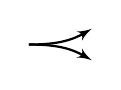
\begin{tikzpicture}[scale=1]
		\coordinate (1) at (0,0);
		\coordinate (2) at (.8,0.2);
		\coordinate (3) at (.8,-0.2);
		\path[thick,-{latex'},out = 0, in = 210] (1) edge (2);
		\path[thick,-{latex'},out = 0, in = 150] (1) edge (3);
		\end{tikzpicture}}
	\hspace{3pt}}


\newcommand{\allconstructions}[1]{\mathbb{C}(#1)} % all constructions in space #1
\newcommand{\constructionofD}[1]{\mathit{con}(#1)}

%%% TransferSchemas %% NO PURGING HERE

\newcommand{\trelation}{R} % term relation
\newcommand{\vtrelation}{R} % variadic term relation
\newcommand{\settrelations}{\mathscr{R}} % set of term relations

\newcommand{\cclass}{\mathscr{G}} % class of constructions

\newcommand{\crelationI}{\trelation_F} % input term relations for tSchema
\newcommand{\crelationO}{\trelation_C} % output relation for tSchema

\newcommand{\tSchemaRels}{(\crelationI,\crelationO)} % the tSchema relation pair

\newcommand{\fcor}[2]{\langle #1, #2 \rangle}

\newcommand{\omittingDiagrams}[2]{\begin{center}
		\begin{tikzpicture}[omitting]
		\node[term = $t$] (v) at (0,5.5) {$v$};
		\node[above left = -0.2cm and 1cm of v] {$#1$};
		\node[omitted, below = of v] (u) {} ;
		\node[term = $t_1$, below left = of u] (v1) {$v_1$};
		\node[below = of u] (d) {$\cdots$};
		\node[term = $t_n$,below right = of u] (vn) {$v_n$};
		\path[->]
		(v1) edge (u)
		(vn) edge (u)
		(u) edge (v)
		;

		\node[term = $t'$, right = 6cm of v] (v2) {$v'$};
		\node[above left = -0.2cm and 1cm of v2] {$#2$};
		\node[omitted, below = of v2] (u2) {} ;
		\node[term = $t_1'$, below left = of u2] (v21) {$v_1'$};
		\node[below = of u2] (d2) {$\cdots$};
		\node[term = $t_m'\,{,}$,below right = of u2] (v2n) {$v_m'$};
		\path[->]
		(v21) edge (u2)
		(v2n) edge (u2)
		(u2) edge (v2)
		;

		%\node at (3.5,7) {$(t,t') \in R$};
		%\node at (3.5,0) {$(t_1,\ldots,t_n,t_1'\ldots,t_m') \in \mathcal{R}$};
		\end{tikzpicture}
	\end{center}}

%%% Patterns %% not fully purged


\newcommand{\pat}{\textup{pat}}
\newcommand{\pattern}{\textup{pattern}} % not used in JAIR

\newcommand{\patterngraphn}{\Gamma}
\newcommand{\pspacen}{\mathcal{P}}
\newcommand{\pspace}{(\tsystemn, \cspecificationn, \patterngraphn)}
\newcommand{\patternn}{P}

\newcommand{\pgraphn}{\gamma}
\newcommand{\ppair}{(\pgraphn,v)}
\newcommand{\ppaird}{(\pgraphn',v')}
\newcommand{\ppairi}{(\pgraphn_i,v_i)}

\newcommand{\setofpatterns}{\mathscr{\patternn}}

\newcommand{\setofmatches}{\mathscr{M}}

\newcommand{\setofpatternsg}{\mathscr{G}}
\newcommand{\setofpatternse}{\mathscr{E}}
\newcommand{\setofpatternsi}{\mathscr{I}}
\newcommand{\setofpatternsssg}{\mathscr{S}}
\newcommand{\setofpatternss}{\mathscr{S}}


\newcommand{\decompositionn}{D}
\newcommand{\pdecompositionn}{\Delta}
\newcommand{\decomposition}{(V,\arrows, \incVert, \lab{A}, \lab{V})}
\newcommand{\decompositiond}{(V',\arrows', \incVert', \lab{A}', \lab{V'})}
\newcommand{\treeroot}[1]{\mathit{root}(#1)}

\DeclareMathOperator{\dec}{Dec}
\newcommand{\dsequence}[1]{\dec(#1)}

\newcommand{\patterntreen}{T}
\newcommand{\patterntree}{(V,\arrows, \incVert\colon \arrows\to V\times V, \lab{A}, \lab{V}')}

\newcommand{\setofpatterntrees}{\mathscr{D}}

\newcommand{\patternlink}{\mathscr{L}}

\newcommand{\foundationrelation}{F}
\newcommand{\constructrelation}{R_t}
\newcommand{\structurerelation}{S_c}

\newcommand{\foundationrelationp}[1]{\foundationrelation(#1)}
\newcommand{\constructrelationp}[1]{\constructrelation(#1)}
\newcommand{\structurerelationp}[1]{\structurerelation(#1)}

\newcommand{\matchesarrow}{\rightsquigarrow}

\newcommand{\descriptionn}{\mathcal{D}}



%%%%%%%%%%%%%%%%%%%%%%%%%%%%%%%%%%%%%%%%%%

\newcommand{\TSGindex}[1]{\mathit{G}_{#1}}
\newcommand{\absindex}[1]{\mathit{term}_{#1}}
\newcommand{\clabelindex}[1]{\mathit{cname}_{#1}}
\newcommand{\ctypeindex}[1]{\mathit{ctype}_{#1}}
\newcommand{\builders}{\mathit{B}}
\newcommand{\entailers}{\mathit{E}}




%%% Vector visualisation
\newcommand{\vectorVis}[2]{%
	\begin{tikzpicture}[scale = #2, >={angle 90}]  %projectile motion
	\draw[very thin, gray!20] (0,0) grid (3.5,3.5);
	\draw[->] (-0.1,0) -- (3.5,0) node[right] {$x$};
	\draw[->] (0,-0.1) -- (0,3.5) node[above] {$y$};
	\draw[->, thick, color=darkblue] (0,0) -- #1 node[above] {};
	\draw[-] (1,-0.1) -- (1,0.1) node[below] {\tiny $1$};
	\draw[-] (2,-0.1) -- (2,0.1) node[below] {\tiny $2$};
	\draw[-] (3,-0.1) -- (3,0.1) node[below] {\tiny $3$};
	%
	\draw[-] (-0.1,1) -- (0.1,1) node[left] {\tiny $1$};
	\draw[-] (-0.1,2) -- (0.1,2) node[left] {\tiny $2$};
	\draw[-] (-0.1,3) -- (0.1,3) node[left] {\tiny $3$};
	\end{tikzpicture}}

\newcommand{\crc}{%
	
\begin{tikzpicture}[inner sep = 0pt]
	\draw (0,0) circle (.07cm);
	\fill[black, opacity = 0.15] (0,0) circle (.07cm);
	\end{tikzpicture}%
}
\newcommand{\oo}{%
	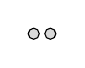
\begin{tikzpicture}[inner sep = 0pt]
	\node[anchor = east] (o1) at (0,0) {\crc};
	\node[anchor = east] (o2) at (6pt,0) {\crc};
	\end{tikzpicture}%
}
\newcommand{\ooo}{%
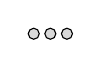
\begin{tikzpicture}[inner sep = 0pt]
\node[anchor = east] (o1) at (0,0) {\crc};
\node[anchor = east] (o2) at (6pt,0) {\crc};
\node[anchor = east] (o2) at (12pt,0) {\crc};
\end{tikzpicture}%
}
\newcommand{\oooo}{%
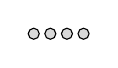
\begin{tikzpicture}[inner sep = 0pt]
\node[anchor = east] (o1) at (0,0) {\crc};
\node[anchor = east] (o2) at (6pt,0) {\crc};
\node[anchor = east] (o2) at (12pt,0) {\crc};
\node[anchor = east] (o2) at (18pt,0) {\crc};
\end{tikzpicture}%
}
\newcommand{\ooV}{%
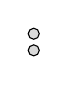
\begin{tikzpicture}[inner sep = 0pt]
\node[anchor = east] (o1) at (0,0) {\crc};
\node[anchor = east] (o2) at (0,6pt) {\crc};
\end{tikzpicture}%
}
\newcommand{\oooV}{%
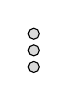
\begin{tikzpicture}[inner sep = 0pt]
\node[anchor = east] (o1) at (0,0) {\crc};
\node[anchor = east] (o2) at (0,6pt) {\crc};
\node[anchor = east] (o2) at (0,12pt) {\crc};
\end{tikzpicture}%
}
\newcommand{\ooooV}{%
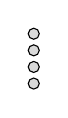
\begin{tikzpicture}[inner sep = 0pt]
\node[anchor = east] (o1) at (0,0) {\crc};
\node[anchor = east] (o2) at (0,6pt) {\crc};
\node[anchor = east] (o2) at (0,12pt) {\crc};
\node[anchor = east] (o2) at (0,18pt) {\crc};
\end{tikzpicture}%
}
